
\subsubsection{Mô tả quá trình phân tích}
\noindent\textbf{1.1.1\quad Mô tả ban đầu}\\
- File cần phân tích: \texttt{CrackThisApp.exe}, đi kèm với thư viện \texttt{CrackThisApp.dll}.\\
- Công cụ sử dụng: \texttt{OllyDbg}, \texttt{IDA Pro}.\\
- Mục đích: Xác định chuỗi 9 số hợp lệ để vượt qua cơ chế bảo vệ của chương trình, sao cho khi chuyển các số này sang mã ASCII, chúng tạo thành một từ tiếng Anh có nghĩa với 9 chữ cái.

\noindent\textbf{1.1.2\quad Phân tích bằng OllyDbg}\\
- Tải \texttt{CrackThisApp.exe} vào \texttt{OllyDbg}, chương trình sẽ nạp thư viện \texttt{CrackThisApp.dll} vào bộ nhớ và thực thi hàm \texttt{\_calc}.
\begin{center}
	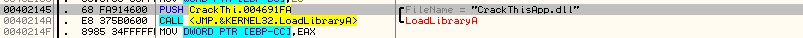
\includegraphics[width=1.0\textwidth]{img/file-1/image1.png}
\end{center}
- Hàm \texttt{\_calc} sẽ thực hiện kiểm tra key và chịu trách nhiệm xử lý logic chính của ứng dụng.
\begin{center}
	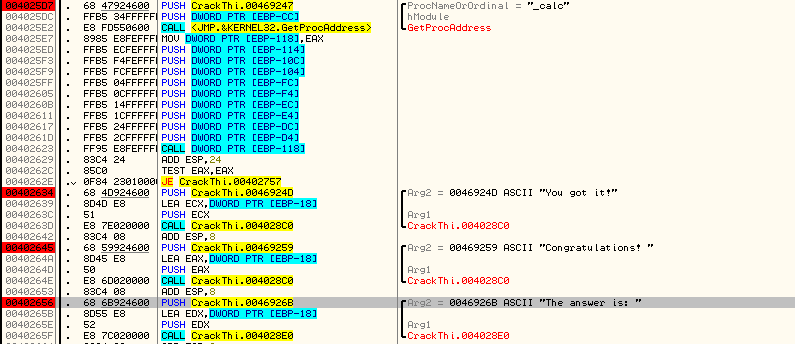
\includegraphics[width=1.0\textwidth]{img/file-1/image2.png}
\end{center}
- Nhấn \texttt{Run} hoặc \texttt{F9} để chạy chương trình và thử nhập 9 số bất kỳ vào ma trận trống. Khi đó chương trình sẽ đọc 9 ô nhập liệu rồi chuyển sang số nguyên để truyền vào hàm \texttt{\_calc}. Sau đó nhấn \texttt{Check} để kiểm tra kết quả. 
\begin{center}
	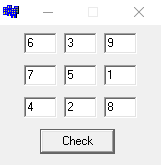
\includegraphics[width=0.3\textwidth]{img/file-1/image3.png}
\end{center}
- Khi nhập sai, chương trình sẽ thông báo không thành công và chuyển hướng đến nhãn \texttt{BadBoy}.
\begin{center}
	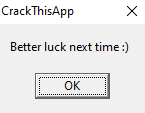
\includegraphics[width=0.3\textwidth]{img/file-1/image4_0.png}
\end{center} 
\begin{center}
	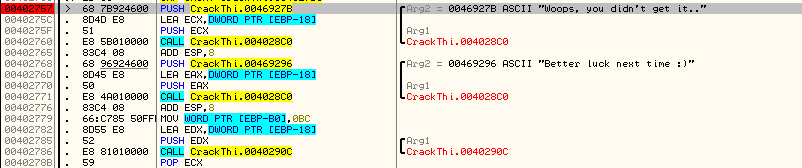
\includegraphics[width=\textwidth]{img/file-1/image4.png}
\end{center}

- Khi ta không nhập hết mà bỏ trống 1 hoặc nhiều ô thì chương trình cũng sẽ xuất thông báo yêu cầu nhập đầy đủ dữ liệu.\\
\begin{center}
	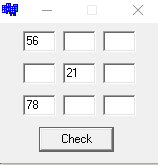
\includegraphics[width=0.3\textwidth]{img/file-1/image12_0.png}
\end{center}   

\begin{center}
	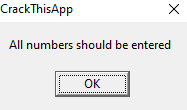
\includegraphics[width=0.4\textwidth]{img/file-1/image12_1.png}
\end{center}  

- Nhận định: Toàn bộ cơ chế xử lý được triển khai trong hàm \texttt{\_calc} của \texttt{CrackThisApp.dll}.

\noindent\textbf{1.1.3\quad Phân tích hàm \texttt{\_calc} bằng IDA Pro}\\
- Nạp \texttt{CrackThisApp.dll} vào \texttt{IDA Pro} để phân tích chi tiết hàm \texttt{\_calc}.
\begin{center}
	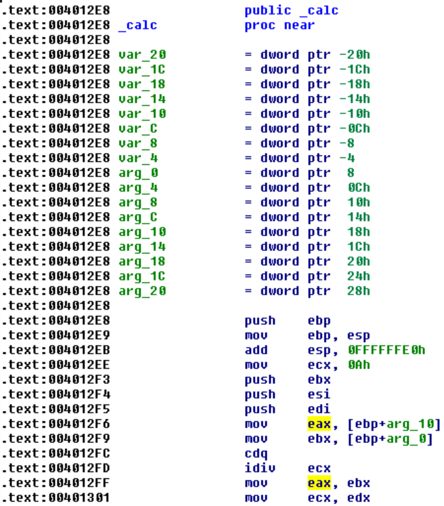
\includegraphics[width=0.8\textwidth]{img/file-1/image5.png}
\end{center}
- Hàm \texttt{\_calc} nhận 9 tham số, được đặt tên lần lượt là \texttt{number1}, \texttt{number2}, ..., \texttt{number9}, tương ứng với 9 số người dùng nhập. \\
- Ở phần đầu hàm, các biến \texttt{var\_20}, \texttt{var\_1C}, \texttt{var\_18}, \texttt{var\_14}, \texttt{var\_10}, \texttt{var\_C}, \texttt{var\_8}, \texttt{var\_4} và các tham số \texttt{arg\_0}, \texttt{arg\_4}, \texttt{arg\_8}, \texttt{arg\_C}, \texttt{arg\_10}, \texttt{arg\_14}, \texttt{arg\_18}, \texttt{arg\_1C}, \texttt{arg\_20} được xác định. \\
- Với 9 tham số bắt đầu bằng \texttt{arg} và cách nhau 4 đơn vị, có thể suy ra đây là 9 số nhập vào, được đổi tên thành \texttt{number1}, \texttt{number2}, \texttt{number3}, ..., \texttt{number9}.\\
\textbf{- Khởi tạo stack frame và lưu trữ thanh ghi}

\begin{lstlisting}
	.text:004012E8 _calc           proc near
	.text:004012E8 var_20          = dword ptr -20h
	.text:004012E8 var_1C          = dword ptr -1Ch
	.text:004012E8 var_18          = dword ptr -18h
	.text:004012E8 var_14          = dword ptr -14h
	.text:004012E8 var_10          = dword ptr -10h
	.text:004012E8 var_C           = dword ptr -0Ch
	.text:004012E8 var_8           = dword ptr -8
	.text:004012E8 var_4           = dword ptr -4
	.text:004012E8 number1         = dword ptr  8
	.text:004012E8 number2         = dword ptr  0Ch
	.text:004012E8 number3         = dword ptr  10h
	.text:004012E8 number4         = dword ptr  14h
	.text:004012E8 number5         = dword ptr  18h
	.text:004012E8 number6         = dword ptr  1Ch
	.text:004012E8 number7         = dword ptr  20h
	.text:004012E8 a8              = dword ptr  24h
	.text:004012E8 number9         = dword ptr  28h
	.text:004012E8
	.text:004012E8                 push    ebp
	.text:004012E9                 mov     ebp, esp
	.text:004012EB                 add     esp, 0FFFFFFE0h
	.text:004012EE                 mov     ecx, 0Ah
	.text:004012F3                 push    ebx
	.text:004012F4                 push    esi
	.text:004012F5                 push    edi
\end{lstlisting}

\textbf{Chức năng}: Thiết lập stack frame cho hàm:
\begin{itemize}
	\item Lưu con trỏ khung stack cũ (\texttt{push ebp; mov ebp, esp}).
	\item Phân bổ 32 byte (0x20) cho các biến cục bộ (\texttt{add esp, 0FFFFFFE0h}).
	\item Lưu các thanh ghi \texttt{ebx}, \texttt{esi}, \texttt{edi} để sử dụng sau này.
	\item Khởi tạo \texttt{ecx = 0Ah} (10), được dùng làm số chia cho các phép tính modulo và chia lấy nguyên.
\end{itemize}

\textbf{- Tính toán các giá trị modulo ban đầu}

\begin{lstlisting}
	.text:004012F6                 mov     eax, [ebp+number5]
	.text:004012F9                 mov     ebx, [ebp+number1]
	.text:004012FC                 cdq
	.text:004012FD                 idiv    ecx
	.text:004012FF                 mov     eax, ebx
	.text:00401301                 mov     ecx, edx
	.text:00401303                 cdq
	.text:00401304                 mov     edi, [ebp+number3]
	.text:00401307                 mov     esi, [ebp+number2]
	.text:0040130A                 push    ecx
	.text:0040130B                 mov     ecx, 0Ah
	.text:00401310                 idiv    ecx
	.text:00401312                 pop     ecx
	.text:00401313                 mov     [ebp+var_4], edx
	.text:00401316                 mov     eax, [ebp+number6]
	.text:00401319                 push    ecx
	.text:0040131A                 cdq
	.text:0040131B                 mov     ecx, 0Ah
	.text:00401320                 idiv    ecx
	.text:00401322                 pop     ecx
	.text:00401323                 mov     [ebp+var_8], edx
	.text:00401326                 mov     eax, esi
	.text:00401328                 push    ecx
	.text:00401329                 cdq
	.text:0040132A                 mov     ecx, 0Ah
	.text:0040132F                 idiv    ecx
	.text:00401331                 pop     ecx
	.text:00401332                 add     edx, 3     ; cong 3
	.text:00401335                 mov     [ebp+var_C], edx
	.text:00401338                 mov     eax, edi
	.text:0040133A                 cdq
	.text:0040133B                 push    ecx
	.text:0040133C                 mov     ecx, 0Ah   ; chia 10 lan 1
	.text:00401341                 idiv    ecx
	.text:00401343                 cdq
	.text:00401344                 pop     ecx
	.text:00401345                 push    ecx
	.text:00401346                 mov     ecx, 0Ah   ; chia 10 lan 2
	.text:0040134B                 idiv    ecx
	.text:0040134D                 pop     ecx
	.text:0040134E                 add     edx, 5     ; cong 5
	.text:00401351                 mov     [ebp+var_10], edx
	.text:00401354                 mov     eax, [ebp+number9]
	.text:00401357                 push    ecx
	.text:00401358                 cdq
	.text:00401359                 mov     ecx, 0Ah  ; chia 10 lan 1
	.text:0040135E                 idiv    ecx
	.text:00401360                 cdq
	.text:00401361                 pop     ecx
	.text:00401362                 push    ecx
	.text:00401363                 mov     ecx, 0Ah  ; chia 10 lan 2
	.text:00401368                 idiv    ecx
	.text:0040136A                 pop     ecx
	.text:0040136B                 mov     [ebp+var_14], edx
	.text:0040136E                 mov     eax, [ebp+number7]
	.text:00401371                 push    ecx
	.text:00401372                 cdq
	.text:00401373                 mov     ecx, 0Ah
	.text:00401378                 idiv    ecx
	.text:0040137A                 pop     ecx
	.text:0040137B                 mov     eax, edx ; number7_mod10
\end{lstlisting}

\textbf{Chức năng}: Tính toán các giá trị modulo và chia lấy nguyên cần thiết cho các công thức:
\begin{itemize}
	\item \texttt{number5 mod 10} (lưu trong \texttt{ecx} tạm thời).
	\item \texttt{number1 mod 10} (lưu trong \texttt{var\_4}).
	\item \texttt{number6 mod 10} (lưu trong \texttt{var\_8}).
	\item \texttt{(number2 mod 10) + 3} (lưu trong \texttt{var\_C}).
	\item \texttt{(\(\lfloor\)number3 / 10\(\rfloor\) mod 10) + 5} (lưu trong \texttt{var\_10})
	\item \texttt{(}\(\lfloor\)\texttt{number9} / 10\(\rfloor\) \texttt{mod 10}\texttt{)} (lưu trong \texttt{var\_14}).
	\item \texttt{number7 mod 10} (lưu trong \texttt{eax}).
\end{itemize}
Các phép chia (\texttt{idiv}) được thực hiện với số chia 10 (\texttt{ecx = 0Ah}), và kết quả modulo được lưu vào các biến cục bộ. Lệnh \texttt{push ecx} và \texttt{pop ecx} được dùng để bảo vệ giá trị \texttt{number5 mod 10}.

\textbf{- Tính toán giá trị \texttt{var\_18}}

\begin{lstlisting}
	.text:0040137D                 mov     edx, ecx ; number5_mod10
	.text:0040137F                 add     eax, 2   ; number7_mod10_cong2
	.text:00401382                 add     edx, edx        ; two fold
	.text:00401384                 lea     edx, [edx+edx*4] ; five fold
	.text:00401387                 add     edx, [ebp+var_4] ; 10 * number5_mod10 + var_4
	.text:0040138A                 add     edx, edx
	.text:0040138C                 lea     edx, [edx+edx*4]
	.text:0040138F                 add     edx, [ebp+var_10] ; 100 * number5_mod10 +
	.text:0040138F                   ; 10 * var_4 +
	.text:0040138F                   ; var_10
	.text:00401392                 add     edx, edx
	.text:00401394                 lea     edx, [edx+edx*4]
	.text:00401397                 add     edx, [ebp+var_14] ; 1000 * number5_mod10 +
	.text:00401397                   ; 100 * var_4 +
	.text:00401397                   ; 10 * var_10 +
	.text:00401397                   ; var_14
	.text:0040139A                 add     edx, edx
	.text:0040139C                 lea     edx, [edx+edx*4]
	.text:0040139F                 add     edx, eax   ; 10000 * number5_mod10 +
	.text:0040139F                   ; 1000 * var_4 +
	.text:0040139F                   ; 100 * var_10 +
	.text:0040139F                   ; 10 * var_14 +
	.text:0040139F                   ; number7_mod10_cong2
	.text:004013A1                 mov     [ebp+var_18], edx
\end{lstlisting}

\textbf{Chức năng}: Tính toán giá trị \texttt{var\_18} theo công thức:\\
\[
\texttt{var\_18} = 10000 \times (\texttt{number5} \bmod 10) + 1000 \times ((\texttt{number2} \bmod 10) + 3) + 100 \times (\lfloor \texttt{number3} / 10 \rfloor \bmod 10) + 5 + 10 \times (\lfloor \texttt{number9} / 10 \rfloor \bmod 10) + (\texttt{number7} \bmod 10) + 2
\]
Các phép nhân được thực hiện bằng cách nhân với 2 (\texttt{add edx, edx}) và cộng với 4 lần giá trị (\texttt{lea edx, [edx+edx*4]}), tương đương nhân với 10. Kết quả cuối cùng được lưu vào \texttt{var\_18}.

\textbf{- Tính toán giá trị \texttt{var\_1C}}

\begin{lstlisting}
	.text:004013A4                 mov     edx, ecx
	.text:004013A6                 add     edx, edx
	.text:004013A8                 add     ecx, ecx
	.text:004013AA                 lea     edx, [edx+edx*4]
	.text:004013AD                 lea     ecx, [ecx+ecx*4]
	.text:004013B0                 add     edx, [ebp+var_8]
	.text:004013B3                 add     edx, edx
	.text:004013B5                 lea     edx, [edx+edx*4]
	.text:004013B8                 add     edx, [ebp+var_10]
	.text:004013BB                 add     edx, edx
	.text:004013BD                 lea     edx, [edx+edx*4]
	.text:004013C0                 add     edx, [ebp+var_14]
	.text:004013C3                 add     edx, edx
	.text:004013C5                 lea     edx, [edx+edx*4]
	.text:004013C8                 add     edx, eax
	.text:004013CA                 mov     [ebp+var_1C], edx
\end{lstlisting}

\textbf{Chức năng}: Tính toán giá trị \texttt{var\_1C} theo công thức:\\
\[
\texttt{var\_1C} = 10000 \times (\texttt{number5} \bmod 10) + 1000 \times (\texttt{number6} \bmod 10) + 100 \times (\lfloor \texttt{number3} / 10 \rfloor \bmod 10) + 5 + 10 \times (\lfloor \texttt{number9} / 10 \rfloor \bmod 10) + (\texttt{number7} \bmod 10) + 2
\]
Tương tự \texttt{var\_18}, nhưng sử dụng \texttt{var\_8} (tức \texttt{number6 mod 10}) thay vì \texttt{var\_4} (tức \texttt{number1 mod 10}). Kết quả được lưu vào \texttt{var\_1C}.

\textbf{- Tính toán giá trị \texttt{var\_20}}
\begin{lstlisting}
	.text:004013CD                 add     ecx, [ebp+var_C]
	.text:004013D0                 mov     edx, ecx
	.text:004013D2                 add     edx, edx
	.text:004013D4                 lea     edx, [edx+edx*4]
	.text:004013D7                 add     edx, [ebp+var_10]
	.text:004013DA                 mov     ecx, edx
	.text:004013DC                 add     ecx, ecx
	.text:004013DE                 lea     ecx, [ecx+ecx*4]
	.text:004013E1                 add     ecx, [ebp+var_14]
	.text:004013E4                 mov     edx, ecx
	.text:004013E6                 add     edx, edx
	.text:004013E8                 lea     edx, [edx+edx*4]
	.text:004013EB                 add     eax, edx
	.text:004013ED                 mov     [ebp+var_20], eax
\end{lstlisting}

\textbf{Chức năng}: Tính toán giá trị \texttt{var\_20} theo công thức:\\
\[
\texttt{var\_20} = 10000 \times (\texttt{number5} \bmod 10) + 1000 \times (\texttt{number1} \bmod 10) + 100 \times (\lfloor \texttt{number3} / 10 \rfloor \bmod 10) + 5 + 10 \times (\lfloor \texttt{number9} / 10 \rfloor \bmod 10) + (\texttt{number7} \bmod 10) + 2
\]

Sử dụng \texttt{var\_C} (tức \texttt{(number2 mod 10) + 3}) thay vì \texttt{var\_4} hoặc \texttt{var\_8}. Kết quả được lưu vào \texttt{var\_20}.

\textbf{- So sánh kết quả và trả về}

\begin{lstlisting}
	.text:0040140B                 call    sub_401478      ; Ham la
	.text:00401410                 add     esp, 24h
	.text:00401413                 cmp     eax, [ebp+var_18]
	.text:00401416                 jnz     short badboy
	.text:00401418 ; .text:00401418
	.text:00401433                 call    sub_401478
	.text:00401438                 add     esp, 24h
	.text:0040143B                 cmp     eax, [ebp+var_1C]
	.text:0040143E                 jnz     short badboy
	.text:00401440 ; .text:00401440
	.text:0040145B                 call    sub_401478
	.text:00401460                 add     esp, 24h
	.text:00401463                 cmp     eax, [ebp+var_20]
	.text:00401466                 jz      short goodboy
	.text:00401468
	.text:00401468 loc_401468:             ; CODE XREF: _calc+12Ej
	.text:00401468                         ; _calc+156j
	.text:00401468                 xor     eax, eax
	.text:0040146A                 jmp     short loc_401471
	.text:0040146C ; ----------------------------------------------------------
	.text:0040146C
	.text:0040146C loc_40146C:            ; CODE XREF: _calc+17Ej
	.text:0040146C                 mov     eax, 1
	.text:00401471
	.text:00401471 loc_401471:            ; CODE XREF: _calc+182j
	.text:00401471                 pop     edi
	.text:00401472                 pop     esi
	.text:00401473                 pop     ebx
	.text:00401474                 mov     esp, ebp
	.text:00401476                 pop     ebp
	.text:00401477                 retn
	.text:00401477 _calc           endp
\end{lstlisting}

\textbf{Chức năng}: So sánh kết quả từ hàm \texttt{sub\_401478} với \texttt{var\_18}, \texttt{var\_1C}, và \texttt{var\_20}:
\begin{itemize}
	\item Gọi \texttt{sub\_401478} và so sánh kết quả với \texttt{var\_18}. Nếu không khớp, nhảy đến \texttt{badboy} (\texttt{xor eax, eax} để trả về 0).
	\item Nếu khớp, gọi lại \texttt{sub\_401478} và so sánh với \texttt{var\_1C}. Nếu không khớp, nhảy đến \texttt{badboy}.
	\item Nếu khớp, gọi \texttt{sub\_401478} lần cuối và so sánh với \texttt{var\_20}. Nếu khớp, nhảy đến \texttt{goodboy} (\texttt{mov eax, 1} để trả về 1).
\end{itemize}
Dọn dẹp stack frame:
\begin{itemize}
	\item Khôi phục các thanh ghi \texttt{edi}, \texttt{esi}, \texttt{ebx}.
	\item Phục hồi stack pointer (\texttt{mov esp, ebp}) và con trỏ khung stack (\texttt{pop ebp}).
\end{itemize}
Trả về giá trị trong \texttt{eax} (0 nếu thất bại, 1 nếu thành công).

\textbf{- So sánh các công thức, ta suy ra điều kiện:}
\[
\text{number1} \mod 10 = \text{number6} \mod 10 = (\text{number2} \mod 10) + 3 \quad (1)
\]

\noindent\textbf{1.1.4\quad Phân tích hàm \texttt{sub\_401478}}\\
- Hàm \texttt{sub\_401478} được gọi để đối chiếu kết quả với \texttt{var\_18}, \texttt{var\_1C}, \texttt{var\_20}.
\begin{center}
	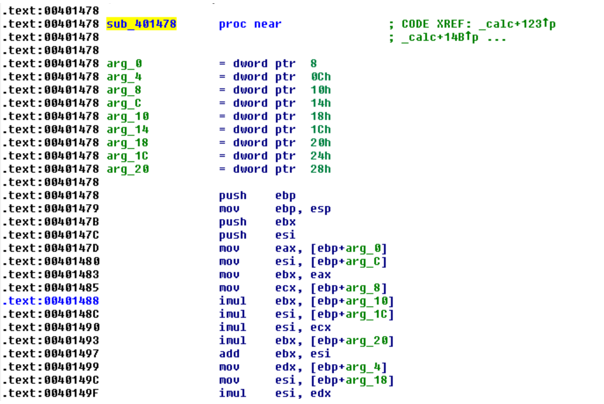
\includegraphics[width=0.8\textwidth]{img/file-1/image6.png}
\end{center}

- Hàm này tái sử dụng các \texttt{arg\_0}, \texttt{arg\_4}, \ldots tương ứng với \texttt{number1}, \texttt{number2}, \ldots \texttt{number9} của hàm \texttt{\_calc}.\\

- Phân tích đoạn mã sau: 
\begin{lstlisting}
	.text:00401478 sub_401478	 proc near               ; CODE XREF: _calc+123p
	.text:00401478                                         ; _calc+14Bp ...
	.text:00401478
	.text:00401478 number1         = dword ptr  8
	.text:00401478 number2         = dword ptr  0Ch
	.text:00401478 number3         = dword ptr  10h
	.text:00401478 number4         = dword ptr  14h
	.text:00401478 number5         = dword ptr  18h
	.text:00401478 number6         = dword ptr  1Ch
	.text:00401478 number7         = dword ptr  20h
	.text:00401478 number8         = dword ptr  24h
	.text:00401478 number9         = dword ptr  28h
	.text:00401478
	.text:00401478                 push    ebp
	.text:00401479                 mov     ebp, esp
	.text:0040147B                 push    ebx
	.text:0040147C                 push    esi
	.text:0040147D                 mov     eax, [ebp+number1]
	.text:00401480                 mov     esi, [ebp+number4]
	.text:00401483                 mov     ebx, eax        ; number1
	.text:00401485                 mov     ecx, [ebp+number3]
	.text:00401488                 imul    ebx, [ebp+number5] ; number1 * number5
	.text:0040148C                 imul    esi, [ebp+number8] ; number4 * number8
	.text:00401490                 imul    esi, ecx        ; number3 * number4 * number8
	.text:00401493                 imul    ebx, [ebp+number9] ; number1 * number5 * number9
	.text:00401497                 add     ebx, esi        ; number1 * number5 * number9 + number3 * number4 * number8
	.text:00401499                 mov     edx, [ebp+number2]
	.text:0040149C                 mov     esi, [ebp+number7]
	.text:0040149F                 imul    esi, edx        ; number2 * number7
	.text:004014A2                 imul    esi, [ebp+number6] ; number2 * number6 * number7
	.text:004014A6                 add     ebx, esi        ;
	.text:004014A6                                         ; number1 * number5 * number9 +
	.text:004014A6                                         ; number2 * number6 * number7 +
	.text:004014A6                                         ; number3 * number4 * number8
	.text:004014A8                 mov     esi, [ebp+number6]
	.text:004014AB                 imul    esi, [ebp+number8]
	.text:004014AF                 imul    esi, eax        ; number1 * number6 * number8
	.text:004014B2                 imul    ecx, [ebp+number5] ; number3 * number5
	.text:004014B6                 mov     eax, [ebp+number9]
	.text:004014B9                 imul    ecx, [ebp+number7] ; number3 * number5 * number7
	.text:004014BD                 imul    edx             ; number2 * number9
	.text:004014BF                 imul    [ebp+number4]   ; number2 * number4 * number9
	.text:004014C2                 add     ecx, esi        ; number1 * number6 * number8 + number3 * number5 * number7
	.text:004014C4                 add     ecx, eax        ;
	.text:004014C4                                         ; number1 * number6 * number8 +
	.text:004014C4                                         ; number2 * number4 * number9 +
	.text:004014C4                                         ; number3 * number5 * number7
	.text:004014C6                 sub     ebx, ecx        ;
	.text:004014C6                                         ; number1 * number5 * number9 +
	.text:004014C6                                         ; number2 * number6 * number7 +
	.text:004014C6                                         ; number3 * number4 * number8 -
	.text:004014C6                                         ; ( number1 * number6 * number8 +
	.text:004014C6                                         ; number2 * number4 * number9 +
	.text:004014C6                                         ; number3 * number5 * number7 )
	.text:004014C8                 mov     eax, ebx
	.text:004014CA                 pop     esi
	.text:004014CB                 pop     ebx
	.text:004014CC                 pop     ebp
	.text:004014CD                 retn
	.text:004014CD sub_401478 endp
\end{lstlisting}
- Từ đoạn mã assembly trên ta suy ra công thức của \texttt{sub\_401478} như sau: \\
\texttt{sub\_401478} = \texttt{number2} * \texttt{number6} * \texttt{number7} \\+ \texttt{number3} * \texttt{number4} * \texttt{number8} \\+ \texttt{number1} * \texttt{number5} * \texttt{number9}\\ - (\texttt{number2} * \texttt{number4} * \texttt{number9}\\ + \texttt{number1} * \texttt{number6} * \texttt{number8}\\ + \texttt{number3} * \texttt{number5} * \texttt{number7}) (2) \\
- Do đó, các số hợp lệ phải đảm bảo \texttt{var\_20}, \texttt{var\_1C}, \texttt{var\_18} và \texttt{sub\_401478} trả về cùng một giá trị.\\
- Điều kiện: \texttt{var\_18} = \texttt{var\_1C} = \texttt{var\_20} = \texttt{sub\_401478}.

\subsubsection{Thuật toán phát sinh khóa}
\noindent\textbf{1.2.1\quad Ý tưởng ban đầu}\\
- Áp dụng phương pháp thử tất cả các trường hợp (brute force) với độ phức tạp \(O(n^9)\) là không thực tế vì có thể mất vài tiếng hoặc nhiều thời gian hơn thế nữa để thực hiện.\\
- Dựa trên điều kiện (1), ta có thể chọn một giá trị ngẫu nhiên bất kỳ cho \texttt{number2}, từ đó tính được \texttt{number1} và \texttt{number6} thoả:
\[
\text{number1}\mod 10 = \text{number6}\mod 10 = (\text{number2}\mod 10) + 3
\]
- Gán các số còn lại bằng \texttt{number2}, sau đó thử các giá trị phù hợp (từ nhỏ đến lớn) cho \texttt{number9} để đáp ứng điều kiện (2). \\
- Nếu không tìm thấy giá trị phù hợp cho \texttt{number9} thì quay lại bước đầu chọn lại \texttt{number2} và làm mới cả quá trình.\\
- Ví dụ một bộ số thỏa mãn: \texttt{39, 36, 12, 12, 12, 39, 12, 12, 863}.
\begin{center}
	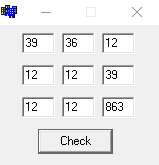
\includegraphics[width=0.3\textwidth]{img/file-1/image11_0.png}
\end{center}

- Kết quả hiển thị thông báo thành công nhưng kèm theo ký tự không rõ nghĩa, cho thấy bộ số này hợp lệ nhưng chưa đáp ứng đầy đủ yêu cầu.
\begin{center}
	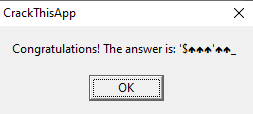
\includegraphics[width=0.4\textwidth]{img/file-1/image11_1.png}
\end{center}

\noindent\textbf{1.2.2\quad Tinh chỉnh thuật toán}\\
- Yêu cầu: Chuỗi số khi chuyển sang mã ASCII phải tạo thành một từ tiếng Anh có nghĩa với 9 chữ cái.\\
- Ví dụ trong bảng ASCII, chẳng hạn mã 77 ứng với ký tự \texttt{H}, 82 ứng với ký tự \texttt{R}...\\
- Chuyển các chữ cái của từ thành mã ASCII, sau đó kiểm tra xem chuỗi số có thỏa mãn các điều kiện (1) và (2) không.\\
- Kết quả: Xác định chuỗi số hợp lệ: \texttt{68, 105, 115, 98, 101, 108, 105, 101, 102}, tương ứng với từ \texttt{Disbelief}.
\begin{center}
	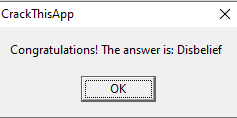
\includegraphics[width=0.4\textwidth]{img/file-1/image9.png}
\end{center}

\subsubsection{Kết luận}
- Ứng dụng sử dụng các phép toán modulo và nhân để xác minh tính hợp lệ của chuỗi số đầu vào.\\
- Kết hợp phân tích mã assembly với từ điển tiếng Anh đã giúp tìm ra chuỗi số thỏa mãn, đồng thời đáp ứng yêu cầu tạo thành một từ tiếng Anh có nghĩa.

\subsubsection{Viết chương trình sinh keygen bằng Python}
\begin{lstlisting}
	def compute_num(num3, num5, num7, num9, digit):
	return 10000 * (num5 % 10) + 1000 * digit + 100 * (int(num3 / 10) % 10 + 5) + 10 * (int(num9 / 10) % 10) + (num7 % 10) + 2
	
	from random import choice
	
	valid = False
	while not valid:
	num2 = 1 + choice(range(100))
	num1 = num6 = num2 + 3
	num3 = num4 = num5 = num7 = num8 = 1 + choice(range(100))
	
	check1 = -1
	check2 = 0
	num9 = 0
	while check1 < check2:
	num9 = num9 + 1
	check1 = verify_num(num1, num2, num3, num4, num5, num6, num7, num8, num9)
	check2 = compute_num(num3, num5, num7, num9, num1 % 10)
	check3 = compute_num(num3, num5, num7, num9, num6 % 10)
	check4 = compute_num(num3, num5, num7, num9, (num2 % 10) + 3)
	
	check1 = verify_num(num1, num2, num3, num4, num5, num6, num7, num8, num9)
	check2 = compute_num(num3, num5, num7, num9, num1 % 10)
	check3 = compute_num(num3, num5, num7, num9, num6 % 10)
	check4 = compute_num(num3, num5, num7, num9, (num2 % 10) + 3)
	
	if check1 == check2 == check3 == check4:
	valid = True
	
	print(num1, num2, num3, num4, num5, num6, num7, num8, num9)
\end{lstlisting} 
	
